\chapter{Experiments}
\label{chap:experiments}

\glsresetall

This chapter presents the experimental study of the \gls{car} method introduced in the previous chapter.
It focuses on evaluating the method's ability to identify conceptual structures.
The remainder of this chapter is organized as follows:
\begin{itemize}
    \item Section~\ref{sec:experiments_software} describes the software implementation of the \gls{car} pipeline.
    \item Section~\ref{sec:experiments_configuration} details the experimental configuration, covering the environments, the \gls{rl} setup, and the surrogate policy training.
    \item Section~\ref{sec:experiments_policy_performance_surrogate_fidelity} presents the training of the initial and surrogate policies and evaluates how faithfully the surrogate policies reproduce the behavior of the initial policy.
    \item Section~\ref{sec:experiments_clustering_quality} provides a quantitative analysis of the \glspl{lr} using the \gls{cu}, \gls{as}, and \gls{acu} metrics.
    \item Section~\ref{sec:experiments_cluster_semantic_interpretation} provides a qualitative analysis of the resulting clusters by manually examining their semantic content.
    \item Section~\ref{sec:experiments_conclusion} summarizes the findings and discusses their implications.
\end{itemize}

\section{Software Implementation}
\label{sec:experiments_software}

This section details the experimental evaluation of the proposed method.
\gls{dl} and \gls{rl} are strongly empirical fields, where experimental evaluation plays an important role in assessing how methods perform in practice.
Particular attention is therefore given to the implementation of \gls{car}.
It relies on established libraries that provide efficient implementations of its main components.
The code is made publicly available as open-source to support reproducible replication of the reported results.\footnote{\url{https://github.com/Maxalaar/Clustering_Agent_Latent_Space}}

The \gls{car} implementation is organized as a pipeline of five stages.
Each stage performs a specific operation and produces the artifacts required by the subsequent stages.
The stages are implemented as independent executables allowing each stage to be rerun independently.
The whole pipeline is driven by a single configuration file, which is the input of the process and gathers the parameters of every stage.
The \gls{car} pipeline is illustrated in Figure~\ref{fig:car_pipeline}, and Table~\ref{tab:software_libraries} summarizes the libraries used throughout the pipeline.
The remainder of this section describes the purpose and implementation of each stage.

\begin{figure}[t]
    \centering
    \resizebox{0.92\textwidth}{!}{
        \begin{tikzpicture}[
            font=\small,
            stage/.style={
                draw, rounded corners=0.15cm, thick,
                minimum width=6cm, minimum height=1.0cm,
                align=center, fill=black!3,
            },
            artifact/.style={align=left, font=\footnotesize\itshape, text=black!65},
            result/.style={align=left, font=\footnotesize, text=black!75},
            flow/.style={-{Latex[length=2.2mm]}, thick},
        ]
            \node[stage] (s1) {\textbf{1. Initial policy training}};
            \node[stage, below=1.5cm of s1] (s2) {\textbf{2. Trajectory dataset generation}};
            \node[stage, below=1.5cm of s2] (s3) {\textbf{3. Surrogate policy training}};
            \node[stage, below=2.0cm of s3] (s4) {\textbf{4. Surrogate policy evaluation}};
            \node[stage, below=1.5cm of s4] (s5) {\textbf{5. Latent space analysis}};

            \draw[flow] (s1) -- (s2);
            \draw[flow] (s2) -- (s3);
            \draw[flow] (s3) -- (s4);
            \draw[flow] (s3.south) -- ++(0,-0.55cm) -| ([xshift=-1.6cm]s5.north);

            \node[artifact] at ($(s1)!0.5!(s2) + (0.3cm,0)$) {initial policy $\OriginalPolicy$};
            \node[artifact] at ($(s2)!0.5!(s3) + (0.3cm,0)$) {trajectory dataset (Parquet)};
            \node[artifact, anchor=west] at ($(s3.south) + (0.3cm,-0.4cm)$) {$n$ surrogate policies $\SurrogatePolicy{1}, \dots, \SurrogatePolicy{n}$};

            % Stage 5 also reuses the trajectory dataset.
            \draw[flow, dashed] (s2.west) -- ++(-1.7cm,0) |- ([yshift=1.5mm]s5.west);
            \node[artifact, anchor=east] at ($(s5.west) + (-1.9cm,0.9cm)$) {trajectory\\ dataset};

            \node[result, anchor=west] at ($(s4.east) + (0.6cm,0)$) {$\rightarrow$~\BehaviorReconstructionName};
            \node[result, anchor=west, text width=4.6cm] at ($(s5.east) + (0.6cm,0)$) {$\rightarrow$~\ClusteringUniversalityName, \AbstractionScoreName, clusters};
        \end{tikzpicture}
    }
    \caption{
        The \gls{car} pipeline. Each stage is an independent executable; stages communicate only through artifacts written to disk (solid arrows). The dashed arrow indicates an artifact reused by a later stage.
    }
    \label{fig:car_pipeline}
\end{figure}


\FloatBarrier

\begin{table}[t]
\hspace*{\fill}
\resizebox{\textwidth}{!}{
\begin{tblr}{|Q[c,m,3.4cm]|Q[c,m,3.5cm]|Q[l,m,8.5cm]|}
    \hline
    \textbf{Pipeline Stage} & \textbf{Library} & \SetCell{c}\textbf{Description} \\
    \hline
    \hline
    \SetCell[r=3]{c} \textbf{Initial policy training} & RLlib \cite{moritz2018ray, liang2018rllib} & Distributed \gls{rl} library used to train the initial policy. \\
    \hline
    & PyTorch \cite{paszke2019pytorch} & Deep learning framework implementing the policy and critic networks. \\
    \hline
    & Gymnasium \cite{towers2024gymnasium} & Common interface used to plug in any \gls{rl} environment. \\
    \hline
    \hline
    \SetCell[r=2]{c} \textbf{Trajectory dataset generation} & RLlib \cite{moritz2018ray, liang2018rllib} & Distributed environment runners used to collect trajectories in parallel. \\
    \hline
    & Apache Arrow \cite{arrow} & Columnar file format (Parquet) used to store the trajectory datasets. \\
    \hline
    \hline
    \textbf{Surrogate policy training} & PyTorch Lightning \cite{falcon2019lightning} & Structured training loop used for the behavior cloning of the surrogate policies. \\
    \hline
    \hline
    \textbf{Surrogate policy evaluation} & RLlib \cite{moritz2018ray, liang2018rllib} & Wraps each surrogate policy as an \gls{rl} policy to evaluate it in the environment. \\
    \hline
    \hline
    \textbf{Latent space analysis} & cuML \cite{raschka2020cuml} & \gls{gpu}-accelerated clustering algorithms used to analyze the latent representations. \\
    \hline
\end{tblr}
}
\hspace*{\fill}
\caption{Main software libraries used at each stage of the \gls{car} pipeline.}
\label{tab:software_libraries}
\end{table}


\subsection{Initial policy training}

The first stage trains the initial policy using RLlib \cite{moritz2018ray, liang2018rllib}.
RLlib provides scalable implementations of \gls{rl} algorithms and supports distributed training.
The use of RLlib also allows \gls{car} to be applied to environments implemented using the Gymnasium interface \cite{towers2024gymnasium}.
By default, the initial policy is trained using \gls{ppo} \cite{schulman2017proximalpolicyoptimizationalgorithms}.
Other RLlib algorithms, such as \gls{appo} \cite{espeholt2018impala}, \gls{dqn} \cite{mnih2013playingatarideepreinforcement}, and DreamerV3 \cite{hafner2023masteringdiversedomainsworld}, can also be selected through the same configuration.

The policy and critic networks are implemented using PyTorch \cite{paszke2019pytorch}.
PyTorch is the standard \gls{dl} framework and is widely used for developing and training \gls{nn}.
It provides \gls{gpu} acceleration and supports a wide range of \gls{nn} architectures.
This makes it well suited for implementing the different policy and critic architectures used in the experiments.

\subsection{Trajectory dataset generation}

The second stage builds the dataset used to train the surrogate policies.
RLlib is used to collect trajectories in parallel using multiple environment runners.
For each step, the dataset stores the observation together with the parameters of the action distribution produced by the initial policy.

Trajectories are stored as Parquet files \cite{arrow}.
Its columnar structure allows efficient data access and supports concurrent processing.
This is useful here because the datasets contain around one million observation--action pairs and cannot be loaded entirely into memory.

\subsection{Surrogate policy training}

The third stage trains the surrogate policies using \gls{bc} on the trajectory dataset.
This provides a supervised learning approach for replicating the initial policy.
The training procedure is implemented using PyTorch Lightning \cite{falcon2019lightning}.
PyTorch Lightning provides a simplified interface for training \gls{nn} with PyTorch.
It handles common training operations such as data loading, optimization, checkpointing, and \gls{gpu} execution.

\subsection{Surrogate policy evaluation}

The fourth stage evaluates how faithfully the surrogate policies reproduce the behavior of the initial policy.
This stage therefore requires both the surrogate policies and the initial policy.
Each surrogate is wrapped as an RLlib policy and evaluated in the original environment.
The initial policy is evaluated under the same conditions to provide the reference return.
The mean cumulative reward of each surrogate over multiple episodes is then compared with that of the initial policy.
Evaluation episodes are collected using parallel environment runners.

This stage computes the \BehaviorReconstructionName.
It therefore verifies that the surrogate policies reproduce the behavior of the initial policy sufficiently well before their \glspl{lr} are analyzed.
If a surrogate does not meet the required level of behavior reconstruction, its training can be repeated.

\subsection{Latent space analysis}

The fifth stage performs the main analysis of \gls{car}.
The trajectory dataset and trained surrogate policies are used to generate the \glspl{lr}.
These representations form the point clouds that are analyzed using clustering algorithms.

The clustering step relies on the cuML library \cite{raschka2020cuml}, which provides \gls{gpu}-accelerated clustering algorithms.
This reduces the computational cost and allows point clouds containing tens of thousands of representations to be analyzed.

The resulting partitions are used to compute the \ClusteringUniversalityName and the \AbstractionScoreName.
The stage also produces the material required for the qualitative analysis, including the clustered point clouds and the cluster assignment of each observation.

\section{Experimental Configuration}
\label{sec:experiments_configuration}

% TODO: describe the experimental setup.
% Points to cover:
% - environments used (Atari benchmark, and any additional environments)
% - reinforcement learning setup: PPO, actor-critic architecture, hyperparameters
% - training of the surrogate policies: dataset size, loss, optimizer, number of epochs
% - training diagnostics: loss curves, reward curves, comparison with benchmark scores

\section{Policy Performance and Surrogate Fidelity}
\label{sec:experiments_policy_performance_surrogate_fidelity}

This section reports the results of training the initial and surrogate policies for \gls{car}, applied to the six environments.
The first part verifies that the initial policies reach a competent level of play and evaluates how faithfully the surrogate policies reproduce their behavior using the \BehaviorReconstructionName.

\subsection{Initial policy training}
\label{ssec:initial_policy_training}

\begin{figure}[t]
    \centering
    \begin{subfigure}[b]{\textwidth}
        \centering
        \captionsetup{skip=2pt}
        \begin{figure}[t]
    \centering
    \resizebox{\textwidth}{!}{
    \begin{tikzpicture}
    \begin{axis}[
        xlabel={Training iteration},
        ylabel={Mean episode return (\% of best reached)},
        grid=major, ymajorgrids=true,
        xmin=0, ymin=0, ymax=105,
        width=\textwidth, height=0.5\textwidth,
        legend style={at={(0.5,-0.22)}, anchor=north, legend columns=3,
            /tikz/every even column/.append style={column sep=0.4cm}},
    ]
        \addplot[color=breakoutColor, mark=\breakoutMark, mark size=\breakoutMarkSize] coordinates {(1,0.1) (211,19.3) (421,19.3) (631,23.6) (841,30.6) (1051,40.7) (1261,52.1) (1471,23.4) (1681,38.3) (1891,58.2) (2101,45.0) (2311,34.8) (2521,55.6) (2731,54.7) (2941,39.5) (3151,68.5) (3361,60.2) (3571,68.8) (3781,42.2) (3991,52.1) (4201,35.7) (4411,45.7) (4621,45.0) (4831,43.5) (5041,53.8) (5050,74.5)};
        \addlegendentry{Breakout}
        \addplot[color=marioBrosColor, mark=\marioBrosMark, mark size=\marioBrosMarkSize] coordinates {(1,0.3) (188,1.3) (375,2.3) (562,6.3) (749,16.5) (936,42.2) (1123,56.5) (1310,68.2) (1497,69.0) (1684,68.8) (1871,73.5) (2058,68.5) (2245,66.9) (2432,61.5) (2619,72.4) (2806,73.5) (2993,70.6) (3180,71.7) (3367,72.3) (3554,72.5) (3741,75.1) (3928,74.9) (4115,80.4) (4302,85.0) (4489,80.4) (4507,84.9)};
        \addlegendentry{Mario Bros}
        \addplot[color=msPacmanColor, mark=\msPacmanMark, mark size=\msPacmanMarkSize] coordinates {(1,0.8) (268,43.8) (535,69.4) (802,87.5) (1069,93.4) (1336,89.3) (1603,95.1) (1870,89.7) (2137,87.2) (2404,88.6) (2671,95.0) (2938,87.7) (3205,92.7) (3472,75.6) (3739,72.9) (4006,74.7) (4273,79.5) (4540,72.3) (4807,73.8) (5074,81.3) (5341,79.6) (5608,69.1) (5875,71.5) (6142,72.7) (6409,70.5) (6425,59.4)};
        \addlegendentry{Ms.\ Pac-Man}
        \addplot[color=pongColor, mark=\pongMark, mark options={line width=1.5pt, scale=1}, mark size=\pongMarkSize] coordinates {(1,0.0) (22,8.9) (43,20.6) (64,47.1) (85,80.8) (106,84.4) (127,87.8) (148,90.1) (169,91.5) (190,92.1) (211,93.0) (232,93.3) (253,94.3) (274,95.3) (295,95.8) (316,96.9) (337,96.4) (358,97.2) (379,97.5) (400,95.6) (421,97.5) (442,98.6) (463,98.7) (484,98.6) (505,99.5) (507,99.3)};
        \addlegendentry{Pong}
        \addplot[color=spaceInvadersColor, mark=\spaceInvadersMark, mark size=\spaceInvadersMarkSize] coordinates {(1,5.3) (192,29.3) (383,42.8) (574,45.6) (765,58.2) (956,51.4) (1147,41.6) (1338,49.8) (1529,56.5) (1720,53.3) (1911,66.3) (2102,66.9) (2293,74.4) (2484,67.1) (2675,66.3) (2866,58.4) (3057,62.3) (3248,72.8) (3439,79.7) (3630,78.2) (3821,81.9) (4012,81.3) (4203,75.6) (4394,81.6) (4585,75.4) (4604,75.7)};
        \addlegendentry{Space Invaders}
        \addplot[color=surroundColor, mark=\surroundMark, mark size=\surroundMarkSize] coordinates {(1,0.0) (298,17.2) (595,24.1) (892,36.6) (1189,33.3) (1486,44.4) (1783,45.6) (2080,60.1) (2377,73.6) (2674,82.8) (2971,87.2) (3268,88.4) (3565,90.0) (3862,92.8) (4159,92.0) (4456,93.6) (4753,95.3) (5050,94.0) (5347,96.4) (5644,95.2) (5941,97.8) (6238,96.0) (6535,96.3) (6832,98.5) (7128,97.9)};
        \addlegendentry{Surround}
    \end{axis}
    \end{tikzpicture}
    }
    \caption{Training of the initial policies with \gls{ppo}, one curve per environment.}
    \label{fig:initial_policy_training}
\end{figure}

        \caption{Training of the initial policies with \gls{ppo}.}
        \label{fig:initial_policy_training}
    \end{subfigure}

    \vspace{2em}

    \begin{subfigure}[b]{\textwidth}
        \centering
        \captionsetup{skip=2pt}
        \begin{figure}[t]
    \centering
    \resizebox{\textwidth}{!}{
    \begin{tikzpicture}
    \begin{axis}[
        ymode=log,
        xlabel={Epoch}, ylabel={Action loss},
        grid=major, ymajorgrids=true,
        xmin=0,
        width=\textwidth, height=0.5\textwidth,
        legend style={at={(0.5,-0.22)}, anchor=north, legend columns=3,
            /tikz/every even column/.append style={column sep=0.4cm}},
    ]
        \addplot[color=breakoutColor, mark=\breakoutMark, mark size=\breakoutMarkSize] coordinates {(1,3.3005) (34,0.7979) (67,0.4972) (100,0.3760) (133,0.3091) (166,0.2642) (199,0.2330) (232,0.2103) (265,0.1923) (298,0.1786) (331,0.1673) (364,0.1578) (397,0.1491) (430,0.1432) (463,0.1361) (496,0.1310) (529,0.1269) (562,0.1226) (595,0.1192) (600,0.1182)};
        \addlegendentry{Breakout}
        \addplot[color=breakoutColor, forget plot] coordinates {(1,3.3093) (34,0.8592) (67,0.5367) (100,0.4015) (133,0.3262) (166,0.2781) (199,0.2438) (232,0.2191) (265,0.2001) (298,0.1841) (331,0.1720) (364,0.1622) (397,0.1531) (430,0.1459) (463,0.1408) (496,0.1356) (529,0.1292) (562,0.1244) (595,0.1218) (600,0.1202)};
        \addplot[color=breakoutColor, forget plot] coordinates {(1,3.3299) (34,0.9590) (67,0.5697) (100,0.4143) (133,0.3293) (166,0.2777) (199,0.2418) (232,0.2167) (265,0.1969) (298,0.1820) (331,0.1700) (364,0.1597) (397,0.1515) (430,0.1439) (463,0.1382) (496,0.1314) (529,0.1275) (562,0.1228) (595,0.1195) (600,0.1184)};

        \addplot[color=marioBrosColor, mark=\marioBrosMark, mark size=\marioBrosMarkSize] coordinates {(1,14.8064) (6,6.6000) (11,4.6932) (16,3.7979) (21,3.2255) (26,2.7950) (31,2.4568) (36,2.1831) (41,1.9586) (46,1.7765) (51,1.6390) (56,1.5198) (61,1.4210) (66,1.3336) (71,1.2585) (76,1.1925) (81,1.1415) (86,1.0899) (91,1.0473) (96,1.0067) (100,0.9770)};
        \addlegendentry{Mario Bros}
        \addplot[color=marioBrosColor, forget plot] coordinates {(1,13.9914) (6,5.7239) (11,4.2091) (16,3.4875) (21,2.9882) (26,2.5980) (31,2.3031) (36,2.0587) (41,1.8517) (46,1.6883) (51,1.5464) (56,1.4302) (61,1.3393) (66,1.2574) (71,1.1879) (76,1.1276) (81,1.0730) (86,1.0292) (91,0.9897) (96,0.9535) (100,0.9291)};
        \addplot[color=marioBrosColor, forget plot] coordinates {(1,14.4070) (6,5.8056) (11,4.3536) (16,3.5892) (21,3.0552) (26,2.6428) (31,2.3269) (36,2.0684) (41,1.8752) (46,1.6995) (51,1.5680) (56,1.4471) (61,1.3526) (66,1.2709) (71,1.1982) (76,1.1348) (81,1.0816) (86,1.0358) (91,0.9926) (96,0.9550) (100,0.9270)};

        \addplot[color=msPacmanColor, mark=\msPacmanMark, mark size=\msPacmanMarkSize] coordinates {(1,27.1299) (12,4.8831) (23,2.4171) (34,1.4646) (45,1.0649) (56,0.8613) (67,0.7298) (78,0.6299) (89,0.5539) (100,0.4961) (111,0.4505) (122,0.4202) (133,0.3914) (144,0.3688) (155,0.3509) (166,0.3339) (177,0.3196) (188,0.3066) (199,0.2941) (200,0.2929)};
        \addlegendentry{Ms.\ Pac-Man}
        \addplot[color=msPacmanColor, forget plot] coordinates {(1,27.4661) (12,4.8214) (23,2.1927) (34,1.5704) (45,1.7119) (56,0.8459) (67,0.6609) (78,0.5625) (89,0.4881) (100,0.4401) (111,0.6438) (122,0.3744) (133,0.3474) (144,0.3299) (155,0.3120) (166,0.2957) (177,0.2860) (188,0.2749) (199,0.3547) (200,0.2608)};
        \addplot[color=msPacmanColor, forget plot] coordinates {(1,27.8892) (12,4.5449) (23,2.2309) (34,1.4869) (45,1.1135) (56,0.8831) (67,0.7563) (78,0.6963) (89,0.5726) (100,0.5595) (111,0.4733) (122,0.4310) (133,0.4060) (144,0.3792) (155,0.3794) (166,0.3522) (177,0.3243) (188,0.3117) (199,0.2987) (200,0.2966)};

        \addplot[color=pongColor, mark=\pongMark, mark options={line width=1.5pt, scale=1}, mark size=\pongMarkSize] coordinates {(1,2.5732) (6,1.3059) (11,0.9484) (16,0.7769) (21,0.6780) (26,0.6095) (31,0.5613) (36,0.5240) (41,0.4939) (46,0.4681) (51,0.4462) (56,0.4273) (61,0.4109) (66,0.3959) (71,0.3829) (76,0.3711) (81,0.3602) (86,0.3497) (91,0.3405) (96,0.3327) (100,0.3266)};
        \addlegendentry{Pong}
        \addplot[color=pongColor, forget plot] coordinates {(1,2.5733) (6,1.3004) (11,0.9744) (16,0.8094) (21,0.7182) (26,0.6519) (31,0.6026) (36,0.5607) (41,0.5261) (46,0.4978) (51,0.4728) (56,0.4510) (61,0.4325) (66,0.4157) (71,0.4007) (76,0.3878) (81,0.3759) (86,0.3657) (91,0.3560) (96,0.3475) (100,0.3415)};
        \addplot[color=pongColor, forget plot] coordinates {(1,2.5732) (6,1.3249) (11,0.9486) (16,0.7818) (21,0.6848) (26,0.6179) (31,0.5676) (36,0.5267) (41,0.4934) (46,0.4651) (51,0.4414) (56,0.4203) (61,0.4020) (66,0.3867) (71,0.3722) (76,0.3598) (81,0.3487) (86,0.3386) (91,0.3294) (96,0.3211) (100,0.3149)};

        \addplot[color=spaceInvadersColor, mark=\spaceInvadersMark, mark size=\spaceInvadersMarkSize] coordinates {(1,2.1788) (12,1.1213) (23,0.9292) (34,0.8281) (45,0.7546) (56,0.6980) (67,0.6508) (78,0.6127) (89,0.5793) (100,0.5531) (111,0.5309) (122,0.5113) (133,0.4946) (144,0.4799) (155,0.4667) (166,0.4549) (177,0.4442) (188,0.4347) (199,0.4264) (200,0.4260)};
        \addlegendentry{Space Invaders}
        \addplot[color=spaceInvadersColor, forget plot] coordinates {(1,2.1801) (12,1.1053) (23,0.9291) (34,0.8288) (45,0.7589) (56,0.7045) (67,0.6616) (78,0.6256) (89,0.5966) (100,0.5717) (111,0.5507) (122,0.5315) (133,0.5150) (144,0.5005) (155,0.4877) (166,0.4762) (177,0.4654) (188,0.4557) (199,0.4471) (200,0.4466)};
        \addplot[color=spaceInvadersColor, forget plot] coordinates {(1,2.1951) (12,1.1148) (23,0.9097) (34,0.8110) (45,0.7429) (56,0.6917) (67,0.6503) (78,0.6153) (89,0.5868) (100,0.5620) (111,0.5397) (122,0.5190) (133,0.5008) (144,0.4857) (155,0.4726) (166,0.4596) (177,0.4486) (188,0.4391) (199,0.4302) (200,0.4298)};

        \addplot[color=surroundColor, mark=\surroundMark, mark size=\surroundMarkSize] coordinates {(1,24.2212) (34,4.7912) (67,2.0912) (100,1.4291) (133,1.1316) (166,0.9598) (199,0.8497) (232,0.7670) (265,0.7080) (298,0.6612) (331,0.6230) (364,0.5919) (397,0.5663) (430,0.5424) (463,0.5225) (496,0.5059) (529,0.4896) (562,0.4765) (595,0.4648) (600,0.4626)};
        \addlegendentry{Surround}
        \addplot[color=surroundColor, forget plot] coordinates {(1,24.0464) (34,2.8642) (67,1.8330) (100,1.3987) (133,1.1628) (166,1.0158) (199,0.9126) (232,0.8353) (265,0.7736) (298,0.7260) (331,0.6858) (364,0.6513) (397,0.6234) (430,0.5987) (463,0.5766) (496,0.5572) (529,0.5407) (562,0.5243) (595,0.5112) (600,0.5088)};
        \addplot[color=surroundColor, forget plot] coordinates {(1,24.7783) (34,4.1007) (67,1.8595) (100,1.3125) (133,1.0589) (166,0.9075) (199,0.8081) (232,0.7370) (265,0.6835) (298,0.6427) (331,0.6093) (364,0.5809) (397,0.5578) (430,0.5374) (463,0.5206) (496,0.5050) (529,0.4904) (562,0.4782) (595,0.4662) (600,0.4658)};
    \end{axis}
    \end{tikzpicture}
    }
    \caption{Training action loss of the surrogate policies.}
    \label{fig:surrogate_policy_training}
\end{figure}

        \caption{Training action loss of the surrogate policies.}
        \label{fig:surrogate_policy_training}
    \end{subfigure}

    \vspace{1em}
    {\hypersetup{pdfborder={0 0 0}}\ref{policyTrainingLegend}}
    \caption{Training of the initial and surrogate policies.}
    \label{fig:policy_training}
\end{figure}


Figure~\ref{fig:initial_policy_training} shows how the initial policies improve during \gls{ppo} training.
For each environment, the mean episode return is normalized so that $0\%$ and $100\%$ correspond to the lowest and highest mean return observed during that run.
In every environment the return increases and then reaches a plateau, at which point training is stopped.
The number of iterations required to reach this plateau varies from a few hundred, for \PongName, to several thousand, for \SurroundName and \MsPacManName.
For the subsequent analysis, the checkpoint with the best performance is retained rather than the final checkpoint.

To confirm that the trained policies play competently, their scores are compared with the reference scores reported by \cite{machado2017revisitingarcadelearningenvironment}.
Each initial policy reaches a score of the same order as these references, so it constitutes a reasonable target for imitation.

\subsection{Surrogate policy training}
\label{ssec:surrogate_policy_training}

Figure~\ref{fig:surrogate_policy_training} shows, for each environment, the training action loss of the three surrogate policies.
In all cases, the loss decreases smoothly, and the three independently trained policies converge to the same value.

We further evaluate the ability of the surrogate policies to replicate the behavior of the initial policies using the \BehaviorReconstructionName (Table~\ref{tab:behavior_reconstruction}).
The surrogate policies reach a \BehaviorReconstructionName of $0.96$ on average over 100 evaluation episodes, ranging from $0.83$ for \BreakoutName to $1.00$ for \MsPacManName and \SurroundName.
They therefore reproduce the decisions of the initial policies closely enough for their latent representations to be analyzed.

\begin{table}[t]
\centering
\resizebox{0.6\linewidth}{!}{
    \begin{tblr}{
        colspec={|c|c|},
        hlines,
        vlines,
        row{1} = {font=\bfseries, halign=c, valign=m}
    }
        Environment     & \textit{Behavior Reconstruction} \\
        \BreakoutName        & 0.83 $\pm$0.03 \\
        \MarioBrosName      & 0.99 $\pm$0.03 \\
        \MsPacManName    & 1.00 $\pm$0.03 \\
        \PongName            & 0.95 $\pm$0.01 \\
        \SpaceInvadersName  & 0.97 $\pm$0.07 \\
        \SurroundName        & 1.00 $\pm$0.01 \\
    \end{tblr}
}
\caption{Evaluation of \BehaviorReconstructionName across the six Atari environments.}
\label{tab:behavior_reconstruction}
\end{table}


\section{Clustering Quality of the Latent Space}
\label{sec:experiments_clustering_quality}

This section analyzes the \gls{ls} of the surrogate policies using \gls{cu}, \gls{as}, and \gls{acu}.
To do so, a random subset of $20\,000$ observations is selected for each environment.
This subset is then embedded into the \gls{ls} of each surrogate policy at each analyzed layer.
This produces a point cloud for each combination of environment, surrogate policy, and layer.
Each point cloud is partitioned using $k$-means clustering \cite{macqueen1967multivariate} for each number of clusters from $2$ to $20$.

The three metrics are then computed from these point clouds and their corresponding clusterings.
Their interpretation, detailed in Section~\ref{sec:clustering_agent_representation_metrics}, is briefly recalled here:
\begin{itemize}
    \item \textbf{\gls{cu}} measures the agreement between the partitions obtained from independently trained surrogate policies.
    A value close to $1$ indicates that the surrogate policies group the observations in the same way, while a value close to $0$ indicates an agreement no better than chance.
    Since it relies on the \gls{ari}, a value of $0.5$ already corresponds to a substantial agreement.
    \item \textbf{\gls{as}} measures how far the latent partitions are from three trivial baselines: the clustering of the raw observations, of the action distribution of the initial policy, and of untrained networks.
    A value close to $1$ indicates that the clusters capture an abstraction learned by the policy, while a value close to $0$ indicates that they merely reproduce one of these baselines.
    \item \textbf{\gls{acu}} subtracts the agreement explained by these baselines from \gls{cu}.
    A value close to $1$ indicates that the surrogate policies converge toward a partition that is both reproducible and non-trivial, providing the strongest support for the \RepresentationConvergenceHypothesisName.
    A value close to $0$, or negative, indicates that the observed agreement is largely explained by the baselines.
\end{itemize}
A high \gls{cu} alone is therefore not sufficient, since it can result from a trivial structure shared by all networks.
It is the combination of a high \gls{cu} and a high \gls{as}, summarized by \gls{acu}, that supports the existence of a stable conceptual organization.

The full results across all environments and analyzed layers are reported in Appendix~\ref{chap:appendix}.
Two complementary analyses are then conducted on these results.
First, the evolution of the three metrics across the different layers is examined to study the effect of representation depth.
Second, for each environment, the layer achieving the highest average \gls{acu} is selected and analyzed in more detail across the different numbers of clusters.

\subsection{Analysis across layers}

The first analysis examines how the three metrics evolve with the depth of the analyzed layer.
For each layer, \gls{cu}, \gls{as}, and \gls{acu} are averaged over the tested cluster numbers.
Figure~\ref{fig:latent_space_curves_by_layer_depth} reports these averages as a function of layer depth.

Across environments, \gls{cu} tends to be highest in the earliest layers and decreases with depth.
\gls{as} follows the opposite trend and generally increases as the representation becomes less tied to the raw observation, the action distribution, and the network's initialization.
This increase is however not monotonic in the deepest layers.
For \MarioBrosName and \MsPacManName, \gls{as} decreases at the last layer, from $0.83$ to $0.68$ and from $0.64$ to $0.60$ respectively, as the latent clustering becomes closer to the clustering of the action distribution, this layer being directly followed by the output layer.
As \gls{acu} combines these two effects, its evolution depends on the environment.

The corresponding linear fits show that \gls{cu} decreases from $0.72$ at the first layer to $0.50$ at the last, with a slope of approximately $-0.04$ per layer, while \gls{as} increases from $0.28$ to $0.69$, with a slope of approximately $+0.06$ per layer.
Over the same range, \gls{acu} increases more moderately from $0.00$ to $0.19$, with a slope of approximately $+0.03$ per layer.
This suggests that, despite the environment-specific variations, deeper representations tend on average to provide a better trade-off between \gls{cu} and \gls{as}.

% Spacing specific to this figure (tuned for its own subfigure heights --
% do not share these with other multi-subfigure figures, see
% figures/clustering_agent_representation/latent_space_curves_by_metric.tex
% and figures/experiments/policy_training.tex for those figures' own copies).
\newcommand{\LatentCurvesByDepthSubfigCaptionSkip}{0.1cm} % space between a subfigure's plot and its own caption
\newcommand{\LatentCurvesByDepthSubfigSpacing}{-0.2cm}   % vertical space between consecutive subfigures
\newcommand{\LatentCurvesByDepthSubfigLegendSpacing}{0.2cm} % vertical space between the last subfigure and the shared legend

\begin{figure}[t]
    \centering
    \begin{subfigure}[b]{\textwidth}
        \centering
        \captionsetup{skip=\LatentCurvesByDepthSubfigCaptionSkip}
        \resizebox{\linewidth}{!}{
        \begin{tikzpicture}
        \begin{axis}[
            xlabel={Layer depth},
            ylabel={\gls{cu}},
            grid=major,
            xmin=1, xmax=8,
            xtick distance=1,
            ymin=0, ymax=1,
            ytick distance=0.25,
            ymajorgrids=true,
            width=\linewidth,
            height=0.33\linewidth,
        ]
            \addplot[color=breakoutColor, mark=\breakoutMark, mark size=\breakoutMarkSize] coordinates {
                (1,0.85) (2,0.73) (3,0.57) (4,0.50) (5,0.50) (6,0.59) (7,0.50) (8,0.51)
            };
            \addplot[color=marioBrosColor, mark=\marioBrosMark, mark size=\marioBrosMarkSize] coordinates {
                (1,0.62) (2,0.68) (3,0.62) (4,0.55) (5,0.55) (6,0.48) (7,0.40) (8,0.37)
            };
            \addplot[color=msPacmanColor, mark=\msPacmanMark, mark size=\msPacmanMarkSize] coordinates {
                (1,0.78) (2,0.72) (3,0.68) (4,0.70) (5,0.70) (6,0.58) (7,0.51) (8,0.58)
            };
            \addplot[color=pongColor, mark=\pongMark, mark size=\pongMarkSize] coordinates {
                (1,0.62) (2,0.65) (3,0.48) (4,0.50) (5,0.50) (6,0.31)
            };
            \addplot[color=spaceInvadersColor, mark=\spaceInvadersMark, mark size=\spaceInvadersMarkSize] coordinates {
                (1,0.75) (2,0.81) (3,0.74) (4,0.63) (5,0.63) (6,0.49)
            };
            \addplot[color=surroundColor, mark=\surroundMark, mark size=\surroundMarkSize] coordinates {
                (1,0.70) (2,0.58) (3,0.66) (4,0.65) (5,0.65) (6,0.59) (7,0.49) (8,0.54)
            };
        \end{axis}
        \end{tikzpicture}
        }
        \caption{\gls{cu} with respect to the layer depth.}
    \end{subfigure}
    \vspace{\LatentCurvesByDepthSubfigSpacing}

    \begin{subfigure}[b]{\textwidth}
        \centering
        \captionsetup{skip=\LatentCurvesByDepthSubfigCaptionSkip}
        \resizebox{\linewidth}{!}{
        \begin{tikzpicture}
        \begin{axis}[
            xlabel={Layer depth},
            ylabel={\gls{as}},
            grid=major,
            xmin=1, xmax=8,
            xtick distance=1,
            ymin=0, ymax=1,
            ytick distance=0.25,
            ymajorgrids=true,
            width=\linewidth,
            height=0.33\linewidth,
        ]
            \addplot[color=breakoutColor, mark=\breakoutMark, mark size=\breakoutMarkSize] coordinates {
                (1,0.15) (2,0.28) (3,0.44) (4,0.76) (5,0.76) (6,0.82) (7,0.79) (8,0.76)
            };
            \addplot[color=marioBrosColor, mark=\marioBrosMark, mark size=\marioBrosMarkSize] coordinates {
                (1,0.44) (2,0.54) (3,0.62) (4,0.66) (5,0.66) (6,0.71) (7,0.87) (8,0.94)
            };
            \addplot[color=msPacmanColor, mark=\msPacmanMark, mark size=\msPacmanMarkSize] coordinates {
                (1,0.19) (2,0.27) (3,0.35) (4,0.41) (5,0.41) (6,0.55) (7,0.64) (8,0.74)
            };
            \addplot[color=pongColor, mark=\pongMark, mark size=\pongMarkSize] coordinates {
                (1,0.33) (2,0.59) (3,0.91) (4,0.95) (5,0.95) (6,0.95)
            };
            \addplot[color=spaceInvadersColor, mark=\spaceInvadersMark, mark size=\spaceInvadersMarkSize] coordinates {
                (1,0.28) (2,0.45) (3,0.54) (4,0.72) (5,0.72) (6,0.74)
            };
            \addplot[color=surroundColor, mark=\surroundMark, mark size=\surroundMarkSize] coordinates {
                (1,0.27) (2,0.45) (3,0.56) (4,0.49) (5,0.49) (6,0.57) (7,0.72) (8,0.77)
            };
        \end{axis}
        \end{tikzpicture}
        }
        \caption{\gls{as} with respect to the layer depth.}
    \end{subfigure}
    \vspace{\LatentCurvesByDepthSubfigSpacing}

    \begin{subfigure}[b]{\textwidth}
        \centering
        \captionsetup{skip=\LatentCurvesByDepthSubfigCaptionSkip}
        \resizebox{\linewidth}{!}{
        \begin{tikzpicture}
        \begin{axis}[
            xlabel={Layer depth},
            ylabel={\gls{acu}},
            grid=major,
            xmin=1, xmax=8,
            xtick distance=1,
            ymin=-0.2, ymax=1,
            ytick distance=0.2,
            ymajorgrids=true,
            width=\linewidth,
            height=0.33\linewidth,
        ]
            \addplot[color=breakoutColor, mark=\breakoutMark, mark size=\breakoutMarkSize] coordinates {
                (1,0.00) (2,0.01) (3,0.01) (4,0.27) (5,0.27) (6,0.41) (7,0.29) (8,0.27)
            };
            \addplot[color=marioBrosColor, mark=\marioBrosMark, mark size=\marioBrosMarkSize] coordinates {
                (1,0.06) (2,0.22) (3,0.24) (4,0.21) (5,0.21) (6,0.19) (7,0.27) (8,0.31)
            };
            \addplot[color=msPacmanColor, mark=\msPacmanMark, mark size=\msPacmanMarkSize] coordinates {
                (1,-0.04) (2,-0.01) (3,0.04) (4,0.10) (5,0.10) (6,0.14) (7,0.15) (8,0.32)
            };
            \addplot[color=pongColor, mark=\pongMark, mark size=\pongMarkSize] coordinates {
                (1,-0.05) (2,0.24) (3,0.39) (4,0.45) (5,0.45) (6,0.27)
            };
            \addplot[color=spaceInvadersColor, mark=\spaceInvadersMark, mark size=\spaceInvadersMarkSize] coordinates {
                (1,0.03) (2,0.25) (3,0.28) (4,0.35) (5,0.35) (6,0.24)
            };
            \addplot[color=surroundColor, mark=\surroundMark, mark size=\surroundMarkSize] coordinates {
                (1,-0.02) (2,0.03) (3,0.22) (4,0.14) (5,0.14) (6,0.16) (7,0.21) (8,0.31)
            };
        \end{axis}
        \end{tikzpicture}
        }
        \caption{\gls{acu} with respect to the layer depth.}
    \end{subfigure}

    \vspace{\LatentCurvesByDepthSubfigLegendSpacing}
    {\hypersetup{pdfborder={0 0 0}}\ref{policyTrainingLegend}}

    \caption{\gls{cu}, \gls{as}, and \gls{acu} averaged over the number of clusters $K \in [2,20]$, with respect to the depth of the analyzed layer, for each of the six environments.}
    \label{fig:latent_space_curves_by_layer_depth}
\end{figure}

% (see Appendix~\ref{chap:appendix} for the full per-layer, per-$K$ values underlying this figure)


\subsection{Analysis of the selected layers}

The second analysis examines the effect of the number of clusters on the three metrics.
For each environment, the layer with the highest average \gls{acu} across the tested cluster numbers is selected.
Table~\ref{tab:latent_space_best_layer} reports the selected layer, together with the corresponding average \gls{cu}, \gls{as}, and \gls{acu}.

Figure~\ref{fig:latent_space_curves_by_metric} reports the evolution of \gls{cu}, \gls{as}, and \gls{acu} as the number of clusters varies.
\PongName achieves the highest average \gls{acu} among the six environments, with a value of $0.45 \pm 0.06$.
This results from a moderate \gls{cu} combined with an \gls{as} that saturates from the third layer onward.
In contrast, \MsPacManName achieves the lowest \gls{as}, with $0.60 \pm 0.05$.
The resulting \gls{acu}, $0.17 \pm 0.06$, is the lowest across the six environments.

The quantitative analysis provides a measure of the consistency and abstraction of the identified clusters, but does not directly reveal their semantic content.
The following section therefore provides a qualitative analysis of the clusters to examine the concepts they represent.

\vspace{1cm}

% Spacing specific to this figure (tuned for its own subfigure heights --
% do not share these with other multi-subfigure figures, see
% figures/experiments/policy_training.tex for that figure's own copies).
\newcommand{\LatentCurvesSubfigCaptionSkip}{0.1cm} % space between a subfigure's plot and its own caption
\newcommand{\LatentCurvesSubfigSpacing}{-0.2cm}   % vertical space between consecutive subfigures
\newcommand{\LatentCurvesSubfigLegendSpacing}{0.2cm} % vertical space between the last subfigure and the shared legend
\newcommand{\LatentCurvesSubfigHeight}{0.33\linewidth} % height of each subfigure's plot (controls this figure's overall scale)

\begin{figure}[H]
    \centering
    \begin{subfigure}[b]{\textwidth}
        \centering
        \captionsetup{skip=\LatentCurvesSubfigCaptionSkip}
        \resizebox{\linewidth}{!}{
        \begin{tikzpicture}
        \begin{axis}[
            xlabel={Number of clusters},
            ylabel={\gls{cu}},
            grid=major,
            xmin=1, xmax=20,
            ymin=0, ymax=1,
            ytick distance=0.25,
            ymajorgrids=true,
            width=\linewidth,
            height=\LatentCurvesSubfigHeight,
        ]
            \addplot[color=breakoutColor, mark=\breakoutMark, mark size=\breakoutMarkSize] coordinates {
                (2,0.66) (3,0.57) (4,0.65) (5,0.79) (6,0.59) (7,0.62) (8,0.56) (9,0.56) (10,0.58) (11,0.64) (12,0.59) (13,0.55) (14,0.55) (15,0.54) (16,0.59) (17,0.60) (18,0.53) (19,0.55) (20,0.55)
            };
            \addplot[color=marioBrosColor, mark=\marioBrosMark, mark size=\marioBrosMarkSize] coordinates {
                (2,0.99) (3,0.84) (4,0.58) (5,0.75) (6,0.54) (7,0.57) (8,0.57) (9,0.66) (10,0.62) (11,0.62) (12,0.58) (13,0.62) (14,0.59) (15,0.55) (16,0.50) (17,0.56) (18,0.59) (19,0.54) (20,0.52)
            };
            \addplot[color=msPacmanColor, mark=\msPacmanMark, mark size=\msPacmanMarkSize] coordinates {
                (2,0.66) (3,0.78) (4,0.58) (5,0.60) (6,0.67) (7,0.64) (8,0.64) (9,0.62) (10,0.59) (11,0.59) (12,0.53) (13,0.62) (14,0.61) (15,0.48) (16,0.48) (17,0.45) (18,0.49) (19,0.48) (20,0.46)
            };
            \addplot[color=pongColor, mark=\pongMark, mark size=\pongMarkSize] coordinates {
                (2,0.60) (3,0.52) (4,0.58) (5,0.49) (6,0.44) (7,0.51) (8,0.58) (9,0.48) (10,0.50) (11,0.52) (12,0.49) (13,0.46) (14,0.50) (15,0.45) (16,0.46) (17,0.47) (18,0.48) (19,0.47) (20,0.53)
            };
            \addplot[color=spaceInvadersColor, mark=\spaceInvadersMark, mark size=\spaceInvadersMarkSize] coordinates {
                (2,0.31) (3,0.73) (4,0.92) (5,0.69) (6,0.61) (7,0.57) (8,0.64) (9,0.61) (10,0.61) (11,0.66) (12,0.58) (13,0.52) (14,0.56) (15,0.63) (16,0.67) (17,0.63) (18,0.63) (19,0.68) (20,0.64)
            };
            \addplot[color=surroundColor, mark=\surroundMark, mark size=\surroundMarkSize] coordinates {
                (2,0.77) (3,0.75) (4,0.67) (5,0.54) (6,0.52) (7,0.55) (8,0.52) (9,0.58) (10,0.61) (11,0.59) (12,0.51) (13,0.52) (14,0.50) (15,0.46) (16,0.50) (17,0.45) (18,0.43) (19,0.43) (20,0.43)
            };
        \end{axis}
        \end{tikzpicture}
        }
        \caption{\gls{cu} with respect to the number of clusters.}
    \end{subfigure}
    \vspace{\LatentCurvesSubfigSpacing}

    \begin{subfigure}[b]{\textwidth}
        \centering
        \captionsetup{skip=\LatentCurvesSubfigCaptionSkip}
        \resizebox{\linewidth}{!}{
        \begin{tikzpicture}
        \begin{axis}[
            xlabel={Number of clusters},
            ylabel={\gls{as}},
            grid=major,
            xmin=1, xmax=20,
            ymin=0, ymax=1,
            ytick distance=0.25,
            ymajorgrids=true,
            width=\linewidth,
            height=\LatentCurvesSubfigHeight,
        ]
            \addplot[color=breakoutColor, mark=\breakoutMark, mark size=\breakoutMarkSize] coordinates {
                (2,0.62) (3,0.83) (4,0.74) (5,0.82) (6,0.85) (7,0.85) (8,0.85) (9,0.85) (10,0.83) (11,0.82) (12,0.85) (13,0.85) (14,0.84) (15,0.83) (16,0.83) (17,0.83) (18,0.84) (19,0.85) (20,0.83)
            };
            \addplot[color=marioBrosColor, mark=\marioBrosMark, mark size=\marioBrosMarkSize] coordinates {
                (2,0.00) (3,0.66) (4,0.63) (5,0.65) (6,0.64) (7,0.62) (8,0.63) (9,0.62) (10,0.69) (11,0.69) (12,0.64) (13,0.66) (14,0.62) (15,0.64) (16,0.67) (17,0.65) (18,0.66) (19,0.64) (20,0.69)
            };
            \addplot[color=msPacmanColor, mark=\msPacmanMark, mark size=\msPacmanMarkSize] coordinates {
                (2,0.56) (3,0.59) (4,0.47) (5,0.57) (6,0.56) (7,0.54) (8,0.55) (9,0.56) (10,0.60) (11,0.58) (12,0.62) (13,0.59) (14,0.59) (15,0.65) (16,0.65) (17,0.68) (18,0.66) (19,0.66) (20,0.67)
            };
            \addplot[color=pongColor, mark=\pongMark, mark size=\pongMarkSize] coordinates {
                (2,0.99) (3,0.99) (4,0.98) (5,0.99) (6,0.97) (7,0.96) (8,0.97) (9,0.96) (10,0.93) (11,0.94) (12,0.96) (13,0.93) (14,0.93) (15,0.93) (16,0.93) (17,0.91) (18,0.90) (19,0.90) (20,0.91)
            };
            \addplot[color=spaceInvadersColor, mark=\spaceInvadersMark, mark size=\spaceInvadersMarkSize] coordinates {
                (2,0.94) (3,0.80) (4,0.69) (5,0.71) (6,0.71) (7,0.75) (8,0.74) (9,0.74) (10,0.75) (11,0.69) (12,0.67) (13,0.68) (14,0.71) (15,0.68) (16,0.68) (17,0.70) (18,0.69) (19,0.74) (20,0.69)
            };
            \addplot[color=surroundColor, mark=\surroundMark, mark size=\surroundMarkSize] coordinates {
                (2,0.66) (3,0.53) (4,0.71) (5,0.70) (6,0.71) (7,0.70) (8,0.71) (9,0.69) (10,0.68) (11,0.71) (12,0.74) (13,0.74) (14,0.73) (15,0.74) (16,0.73) (17,0.75) (18,0.76) (19,0.75) (20,0.76)
            };
        \end{axis}
        \end{tikzpicture}
        }
        \caption{\gls{as} with respect to the number of clusters.}
    \end{subfigure}
    \vspace{\LatentCurvesSubfigSpacing}

    \begin{subfigure}[b]{\textwidth}
        \centering
        \captionsetup{skip=\LatentCurvesSubfigCaptionSkip}
        \resizebox{\linewidth}{!}{
        \begin{tikzpicture}
        \begin{axis}[
            xlabel={Number of clusters},
            ylabel={\gls{acu}},
            grid=major,
            xmin=1, xmax=20,
            ymin=-0.2, ymax=1,
            ytick distance=0.2,
            ymajorgrids=true,
            width=\linewidth,
            height=\LatentCurvesSubfigHeight,
        ]
            \addplot[color=breakoutColor, mark=\breakoutMark, mark size=\breakoutMarkSize] coordinates {
                (2,0.28) (3,0.40) (4,0.39) (5,0.61) (6,0.43) (7,0.47) (8,0.41) (9,0.41) (10,0.42) (11,0.46) (12,0.45) (13,0.40) (14,0.39) (15,0.37) (16,0.42) (17,0.43) (18,0.36) (19,0.40) (20,0.38)
            };
            \addplot[color=marioBrosColor, mark=\marioBrosMark, mark size=\marioBrosMarkSize] coordinates {
                (2,0.00) (3,0.50) (4,0.21) (5,0.40) (6,0.18) (7,0.20) (8,0.20) (9,0.27) (10,0.31) (11,0.31) (12,0.23) (13,0.28) (14,0.21) (15,0.19) (16,0.16) (17,0.22) (18,0.25) (19,0.18) (20,0.21)
            };
            \addplot[color=msPacmanColor, mark=\msPacmanMark, mark size=\msPacmanMarkSize] coordinates {
                (2,0.22) (3,0.37) (4,0.05) (5,0.16) (6,0.23) (7,0.18) (8,0.19) (9,0.19) (10,0.19) (11,0.17) (12,0.15) (13,0.21) (14,0.20) (15,0.13) (16,0.12) (17,0.13) (18,0.15) (19,0.14) (20,0.13)
            };
            \addplot[color=pongColor, mark=\pongMark, mark size=\pongMarkSize] coordinates {
                (2,0.59) (3,0.51) (4,0.56) (5,0.48) (6,0.41) (7,0.48) (8,0.56) (9,0.44) (10,0.44) (11,0.46) (12,0.45) (13,0.40) (14,0.43) (15,0.38) (16,0.39) (17,0.38) (18,0.38) (19,0.38) (20,0.44)
            };
            \addplot[color=spaceInvadersColor, mark=\spaceInvadersMark, mark size=\spaceInvadersMarkSize] coordinates {
                (2,0.26) (3,0.53) (4,0.61) (5,0.40) (6,0.32) (7,0.32) (8,0.38) (9,0.36) (10,0.35) (11,0.35) (12,0.26) (13,0.20) (14,0.27) (15,0.31) (16,0.36) (17,0.33) (18,0.32) (19,0.43) (20,0.34)
            };
            \addplot[color=surroundColor, mark=\surroundMark, mark size=\surroundMarkSize] coordinates {
                (2,0.42) (3,0.28) (4,0.38) (5,0.24) (6,0.23) (7,0.24) (8,0.23) (9,0.27) (10,0.29) (11,0.30) (12,0.24) (13,0.26) (14,0.23) (15,0.20) (16,0.23) (17,0.20) (18,0.18) (19,0.18) (20,0.19)
            };
        \end{axis}
        \end{tikzpicture}
        }
        \caption{\gls{acu} with respect to the number of clusters.}
    \end{subfigure}

    \vspace{\LatentCurvesSubfigLegendSpacing}
    {\hypersetup{pdfborder={0 0 0}}\ref{policyTrainingLegend}}

    \caption{\gls{cu}, \gls{as}, and \gls{acu} with respect to the number of clusters, for each of the six environments, for the layer that maximizes the average \gls{acu} in that environment.}
    \label{fig:latent_space_curves_by_metric}
\end{figure}

% (see Table~\ref{tab:latent_space_best_layer} for the specific layer and average values of each environment)

\begin{table}[t]
\centering
\resizebox{0.8\linewidth}{!}{
    \begin{tblr}{
        colspec={|c|c|c|c|c|},
        hlines,
        vlines,
        row{1} = {font=\bfseries, halign=c, valign=m}
    }
        Environment     & Layer & \gls{cu}        & \gls{as}        & \gls{acu}       \\
        Breakout        & 6b    & 0.59 $\pm$0.06  & 0.82 $\pm$0.05  & 0.41 $\pm$0.06  \\
        Mario Bros      & 8b    & 0.37 $\pm$0.08  & 0.94 $\pm$0.02  & 0.31 $\pm$0.08  \\
        Ms.\ Pac-Man    & 8b    & 0.58 $\pm$0.08  & 0.74 $\pm$0.05  & 0.32 $\pm$0.07  \\
        Pong            & 4     & 0.50 $\pm$0.04  & 0.95 $\pm$0.03  & 0.45 $\pm$0.07  \\
        Space Invaders  & 4     & 0.63 $\pm$0.11  & 0.73 $\pm$0.06  & 0.35 $\pm$0.09  \\
        Surround        & 8b    & 0.54 $\pm$0.10  & 0.77 $\pm$0.07  & 0.31 $\pm$0.06  \\
    \end{tblr}
}
\caption{Layer that maximizes the average \gls{acu} across $K \in [2,20]$ for each environment, together with the corresponding average \gls{cu}, \gls{as}, and \gls{acu} over $K$.}
\label{tab:latent_space_best_layer}
\end{table}

\section{Semantic Interpretation of the Clusters}
\label{sec:experiments_cluster_semantic_interpretation}

The metrics reported in Section~\ref{sec:experiments_clustering_quality} evaluate the \gls{ls} clusterings quantitatively but do not indicate what the resulting clusters actually represent.
This section complements them with a qualitative, hand-labeled inspection of the clusters obtained for each environment.

For each environment, two clusterings are selected for the qualitative analysis.
They are obtained using two different numbers of clusters and may correspond to different layers of the network.
The choice of the layer and the number of clusters is based on the following criteria:
\begin{itemize}
\item \textbf{High \gls{acu}:} The selected clustering should achieve a sufficiently high \gls{acu}, indicating a good balance between consistency and abstraction.
\item \textbf{Manual analysis:} The number of clusters must remain small enough to allow the resulting clusters to be examined manually.
\item \textbf{Limited use of two-cluster partitions:} Clusterings with two clusters often achieve a high \gls{acu}, but provide limited information about the organization of the \gls{ls}. Therefore, at most one of the two selected clusterings uses two clusters, while the other uses a larger number of clusters to provide a more detailed view of the latent space.
\end{itemize}

\newcommand{\qualitativeClusterImageScale}{0.20}

\newlength{\qualitativeClusterImageWidth}
\settowidth{\qualitativeClusterImageWidth}{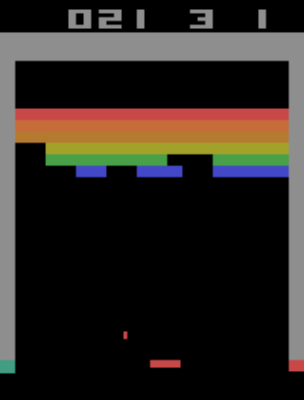
\includegraphics[scale=\qualitativeClusterImageScale]{figures/clustering_agent_representation/pictures/breakout/qualitative/cluster_0/image_1.png}}

% Spacing between the two screenshots of a same cluster.
\newlength{\qualitativeClusterImageGap}
\setlength{\qualitativeClusterImageGap}{0.1cm}

% Spacing between two clusters on the same row of a figure.
\newlength{\qualitativeClusterGap}
\setlength{\qualitativeClusterGap}{0.4cm}

% Vertical spacing between two rows of clusters in a same figure.
\newlength{\qualitativeClusterRowGap}
\setlength{\qualitativeClusterRowGap}{0.3cm}

% The gap is inserted before every cluster except the first one of a figure, so that
% no row carries a trailing gap and every row is centered on the same axis.
\newif\ifqualitativeFirstCluster

% Start of every cluster figure: centers the clusters and applies the row spacing.
\newcommand{\qualitativeClusterFigureSetup}{%
    \centering
    \setlength{\lineskiplimit}{1000pt}%
    \setlength{\lineskip}{\qualitativeClusterRowGap}%
    \qualitativeFirstClustertrue
}

% A cluster shown with two example screenshots, always kept on the same line, labeled with a letter.
\newcommand{\qualitativeClusterTwo}[3]{%
    \ifqualitativeFirstCluster\qualitativeFirstClusterfalse\else\hspace{\qualitativeClusterGap}\fi
    \begin{minipage}[t]{\dimexpr 2\qualitativeClusterImageWidth+\qualitativeClusterImageGap\relax}
        \centering
        \includegraphics[scale=\qualitativeClusterImageScale]{#1}\hspace{\qualitativeClusterImageGap}\includegraphics[scale=\qualitativeClusterImageScale]{#2}\par
        \small\textbf{#3}
    \end{minipage}%
}

\newpage
\subsection{\BreakoutName}

Two clusterings are examined for \BreakoutName (Table~\ref{tab:qualitative_breakout_metrics}), obtained at layer 4 with $K=2$ and at layer 6b with $K=5$.

At layer 4 (Figure~\ref{fig:qualitative_breakout_alt}), the partition captures the position of the ball relative to the brick wall.
The ball remains below the wall in cluster A.
The ball has passed behind the wall in cluster B, allowing it to continue clearing bricks without further interaction with the paddle.

At layer 6b (Figure~\ref{fig:qualitative_breakout}), the partition again isolates situations in which the ball has passed behind the wall in cluster E.
It also identifies the digging of a tunnel through the left side of the wall in cluster C.
Finally, it distinguishes different paddle positions at the beginning of the episode in clusters D, F, and G.

The clustering at layer 4 with $K=2$ is almost perfectly reproducible across surrogate policies, with a \gls{cu} of $0.99$ and an \gls{acu} of $0.87$.
The clustering at layer 6b with $K=5$ is less consistent, with a \gls{cu} of $0.79$ and an \gls{acu} of $0.61$, but reveals additional information about the organization of the \gls{ls}.

\vfill
\begin{table}[H]
    \centering
    \begin{tblr}{
        width=\linewidth,
        colspec={Q[c,wd=1.6cm] X[l]},
        cells = {valign=m},
        rowsep=2pt,
        hline{1,Z} = {1pt},
        hline{4} = {0.5pt},
        hline{2,5} = {0.3pt},
        row{1,4} = {bg=black!8, font=\bfseries},
        column{1} = {font=\bfseries}
    }
        \SetCell[c=2]{l} \makebox[1.9cm][l]{Layer 4}\makebox[1.4cm][l]{$K=2$}\makebox[2.75cm][l]{\gls{cu} 0.99}\makebox[2.75cm][l]{\gls{as} 0.88}\gls{acu} 0.87 & \\
        A & The ball is below the brick wall. \\
        B & The ball passes behind the brick wall. \\
        \SetCell[c=2]{l} \makebox[1.9cm][l]{Layer 6b}\makebox[1.4cm][l]{$K=5$}\makebox[2.75cm][l]{\gls{cu} 0.79}\makebox[2.75cm][l]{\gls{as} 0.82}\gls{acu} 0.61 & \\
        C & Digging a tunnel through the left side of the wall. \\
        D & Start of the episode, paddle on the right. \\
        E & The ball is behind the brick wall. \\
        F & Start of the episode, paddle in the middle. \\
        G & Start of the episode, paddle on the left. \\
    \end{tblr}
    \caption{\gls{cu}, \gls{as}, and \gls{acu} of the two clusterings analyzed in the \BreakoutName environment.}
    \label{tab:qualitative_breakout_metrics}
\end{table}
\vfill

\newpage
\vspace*{\fill}
\begin{figure}[H]
    \qualitativeClusterFigureSetup
    \qualitativeClusterTwo
        {figures/clustering_agent_representation/pictures/breakout/qualitative_alt/cluster_0/image_1.png}
        {figures/clustering_agent_representation/pictures/breakout/qualitative_alt/cluster_0/image_2.png}
        {A}
    \qualitativeClusterTwo
        {figures/clustering_agent_representation/pictures/breakout/qualitative_alt/cluster_1/image_1.png}
        {figures/clustering_agent_representation/pictures/breakout/qualitative_alt/cluster_1/image_2.png}
        {B}
    \caption{Clusters A--B identified by \gls{car} in the \BreakoutName environment (layer 4, $K=2$).}
    \label{fig:qualitative_breakout_alt}
\end{figure}


\begin{figure}[H]
    \qualitativeClusterFigureSetup
    \qualitativeClusterTwo
        {figures/clustering_agent_representation/pictures/breakout/qualitative/cluster_0/image_1.png}
        {figures/clustering_agent_representation/pictures/breakout/qualitative/cluster_0/image_2.png}
        {C}
    \qualitativeClusterTwo
        {figures/clustering_agent_representation/pictures/breakout/qualitative/cluster_1/image_1.png}
        {figures/clustering_agent_representation/pictures/breakout/qualitative/cluster_1/image_2.png}
        {D}
    \qualitativeClusterTwo
        {figures/clustering_agent_representation/pictures/breakout/qualitative/cluster_2/image_1.png}
        {figures/clustering_agent_representation/pictures/breakout/qualitative/cluster_2/image_2.png}
        {E}
    \qualitativeClusterTwo
        {figures/clustering_agent_representation/pictures/breakout/qualitative/cluster_3/image_1.png}
        {figures/clustering_agent_representation/pictures/breakout/qualitative/cluster_3/image_2.png}
        {F}
    \qualitativeClusterTwo
        {figures/clustering_agent_representation/pictures/breakout/qualitative/cluster_4/image_1.png}
        {figures/clustering_agent_representation/pictures/breakout/qualitative/cluster_4/image_2.png}
        {G}
    \caption{Clusters C--G identified by \gls{car} in the \BreakoutName environment (layer 6b, $K=5$).}
    \label{fig:qualitative_breakout}
\end{figure}

\vfill

\newpage
\subsection{\MarioBrosName}

Two clusterings are examined for \MarioBrosName (Table~\ref{tab:qualitative_mario_bros_metrics}), both obtained at layer 3, with $K=3$ and $K=5$.

With $K=3$ (Figure~\ref{fig:qualitative_mario_bros}), the partition is organized around the location of the action.
Mario fights enemies on the left side of the screen in (cluster A).
He fights enemies on the right side of the screen in (cluster C).
The POW block is present in (cluster B), isolating a fixed and recognizable element of the level.

With $K=5$ (Figure~\ref{fig:qualitative_mario_bros_alt}), the partition provides a more detailed description of the situations occurring in the level.
Mario is on the top-left platform in (cluster D).
Mario attacks enemies at the top left in (cluster F).
Mario hits enemies from below in (cluster H).
Mario simply moves through the level in (cluster G).
The POW block remains isolated in (cluster E).

Increasing $K$ from $3$ to $5$ lowers \gls{cu} from $0.84$ to $0.75$.
The \gls{as} remains nearly unchanged, with values of $0.66$ and $0.65$.
This results in a decrease in \gls{acu} from $0.50$ to $0.40$.

\vfill
\begin{table}[H]
    \centering
    \begin{tblr}{
        width=\linewidth,
        colspec={Q[c,wd=1.6cm] X[l]},
        cells = {valign=m},
        rowsep=2pt,
        hline{1,Z} = {1pt},
        hline{5} = {0.5pt},
        hline{2,6} = {0.3pt},
        row{1,5} = {bg=black!8, font=\bfseries},
        column{1} = {font=\bfseries}
    }
        \SetCell[c=2]{l} \makebox[1.9cm][l]{Layer 3}\makebox[1.4cm][l]{$K=3$}\makebox[2.75cm][l]{\gls{cu} 0.84}\makebox[2.75cm][l]{\gls{as} 0.66}\gls{acu} 0.50 & \\
        A & Mario fights enemies on the left side of the screen. \\
        B & The POW block is present. \\
        C & Mario fights enemies on the right side of the screen. \\
        \SetCell[c=2]{l} \makebox[1.9cm][l]{Layer 3}\makebox[1.4cm][l]{$K=5$}\makebox[2.75cm][l]{\gls{cu} 0.75}\makebox[2.75cm][l]{\gls{as} 0.65}\gls{acu} 0.40 & \\
        D & Mario is on the top-left platform. \\
        E & The POW block is present. \\
        F & Mario attacks the enemies at the top right. \\
        G & Mario moves through the level. \\
        H & Mario hits enemies from below on the left side. \\
    \end{tblr}
    \caption{\gls{cu}, \gls{as}, and \gls{acu} of the two clusterings analyzed in the \MarioBrosName environment.}
    \label{tab:qualitative_mario_bros_metrics}
\end{table}
\vfill

\newpage
\vspace*{\fill}
\begin{figure}[H]
    \qualitativeClusterFigureSetup
    \qualitativeClusterTwo
        {figures/clustering_agent_representation/pictures/mario_bros/qualitative/cluster_0/image_1.png}
        {figures/clustering_agent_representation/pictures/mario_bros/qualitative/cluster_0/image_2.png}
        {A}
    \qualitativeClusterTwo
        {figures/clustering_agent_representation/pictures/mario_bros/qualitative/cluster_1/image_1.png}
        {figures/clustering_agent_representation/pictures/mario_bros/qualitative/cluster_1/image_2.png}
        {B}
    \qualitativeClusterTwo
        {figures/clustering_agent_representation/pictures/mario_bros/qualitative/cluster_2/image_1.png}
        {figures/clustering_agent_representation/pictures/mario_bros/qualitative/cluster_2/image_2.png}
        {C}
    \caption{Clusters A--C identified by \gls{car} in the \MarioBrosName environment (layer 3, $K=3$).}
    \label{fig:qualitative_mario_bros}
\end{figure}


\begin{figure}[H]
    \qualitativeClusterFigureSetup
    \qualitativeClusterTwo
        {figures/clustering_agent_representation/pictures/mario_bros/qualitative_alt/cluster_0/image_1.png}
        {figures/clustering_agent_representation/pictures/mario_bros/qualitative_alt/cluster_0/image_2.png}
        {D}
    \qualitativeClusterTwo
        {figures/clustering_agent_representation/pictures/mario_bros/qualitative_alt/cluster_1/image_1.png}
        {figures/clustering_agent_representation/pictures/mario_bros/qualitative_alt/cluster_1/image_2.png}
        {E}
    \qualitativeClusterTwo
        {figures/clustering_agent_representation/pictures/mario_bros/qualitative_alt/cluster_2/image_1.png}
        {figures/clustering_agent_representation/pictures/mario_bros/qualitative_alt/cluster_2/image_2.png}
        {F}
    \qualitativeClusterTwo
        {figures/clustering_agent_representation/pictures/mario_bros/qualitative_alt/cluster_3/image_1.png}
        {figures/clustering_agent_representation/pictures/mario_bros/qualitative_alt/cluster_3/image_2.png}
        {G}
    \caption{Clusters D--G identified by \gls{car} in the \MarioBrosName environment (layer 8b, $K=4$).}
    \label{fig:qualitative_mario_bros_alt}
\end{figure}

\vfill

\newpage
\subsection{\MsPacManName}

Two clusterings are examined for \MsPacManName (Table~\ref{tab:qualitative_ms_pacman_metrics}), obtained at layer 6b with $K=3$ and at layer 4 with $K=5$.

With $K=3$ (Figure~\ref{fig:qualitative_ms_pacman}), the partition captures the progress and state of the game rather than a specific spatial feature of the observation.
The start of the episode is captured in cluster B.
The middle of the episode is captured in cluster A.
The end of the episode is captured in cluster C.

With $K=5$ (Figure~\ref{fig:qualitative_ms_pacman_alt}), the partition provides a more detailed description of the episode.
The initial animation, during which the character cannot move, is isolated in cluster H.
The beginning of actual play is captured in cluster F.
A situation specific to the game mechanics, in which Pac-Man is in booster mode and waits in front of the ghost spawn to eat the ghosts, is isolated in cluster D.
The end of the episode, when at most one power pellet remains, is separated into two similar clusters, E and G.

The two clusterings have the same \gls{cu} of $0.88$.
The clustering at layer 4 has a lower \gls{as} of $0.47$ compared with $0.52$ at layer 6b.
This results in a lower \gls{acu} of $0.35$ compared with $0.40$.

\vfill
\begin{table}[H]
    \centering
    \begin{tblr}{
        width=\linewidth,
        colspec={Q[c,wd=1.6cm] X[l]},
        cells = {valign=m},
        rowsep=2pt,
        hline{1,Z} = {1pt},
        hline{5} = {0.5pt},
        hline{2,6} = {0.3pt},
        row{1,5} = {bg=black!8, font=\bfseries},
        column{1} = {font=\bfseries}
    }
        \SetCell[c=2]{l} \makebox[1.9cm][l]{Layer 6b}\makebox[1.4cm][l]{$K=3$}\makebox[2.75cm][l]{\gls{cu} 0.88}\makebox[2.75cm][l]{\gls{as} 0.52}\gls{acu} 0.40 & \\
        A & Middle of the episode. \\
        B & Start of the episode. \\
        C & End of the episode. \\
        \SetCell[c=2]{l} \makebox[1.9cm][l]{Layer 4}\makebox[1.4cm][l]{$K=5$}\makebox[2.75cm][l]{\gls{cu} 0.88}\makebox[2.75cm][l]{\gls{as} 0.47}\gls{acu} 0.35 & \\
        D & Pac-Man is in booster mode and waits in front of the ghost spawn to eat the ghosts. \\
        E & End of the episode, at most one power pellet remains (similar to cluster G). \\
        F & Start of the episode. \\
        G & End of the episode, at most one power pellet remains (similar to cluster E). \\
        H & Start-of-episode animation, the character cannot move. \\
    \end{tblr}
    \caption{\gls{cu}, \gls{as}, and \gls{acu} of the two clusterings analyzed in the \MsPacManName environment.}
    \label{tab:qualitative_ms_pacman_metrics}
\end{table}
\vfill

\newpage
\vspace*{\fill}
\begin{figure}[t]
    \centering
    \resizebox{\textwidth}{!}{
    \begin{tikzpicture}

    \node (ligne_1) at (0, 0) {};

    \node[] at ($(ligne_1) + (-4.5cm, 0cm)$) {
    \begin{minipage}{4.5cm}
        \centering
        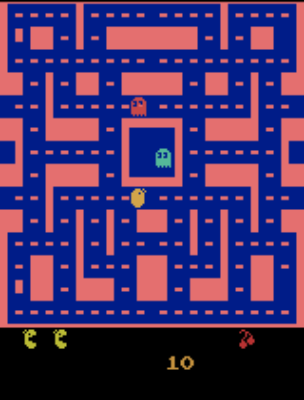
\includegraphics[width=2cm]{figures/clustering_agent_representation/pictures/ms_pacman/qualitative/cluster_1/image_1.png}
        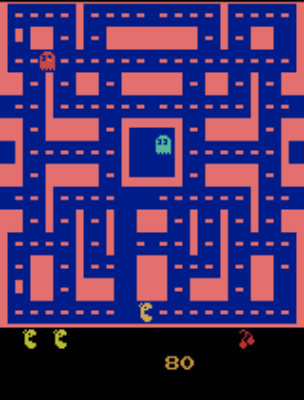
\includegraphics[width=2cm]{figures/clustering_agent_representation/pictures/ms_pacman/qualitative/cluster_1/image_2.png}

        \small Start of the episode.
    \end{minipage}
    };

    \node[] at ($(ligne_1) + (0cm, 0cm)$) {
    \begin{minipage}{4.5cm}
        \centering
        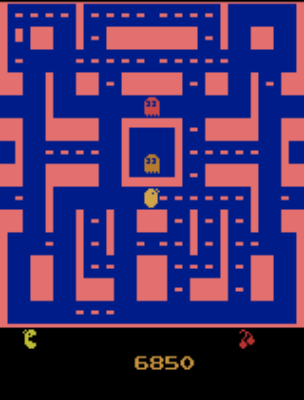
\includegraphics[width=2cm]{figures/clustering_agent_representation/pictures/ms_pacman/qualitative/cluster_0/image_1.png}
        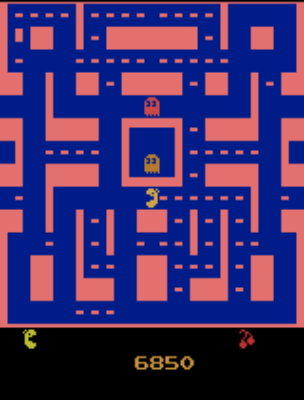
\includegraphics[width=2cm]{figures/clustering_agent_representation/pictures/ms_pacman/qualitative/cluster_0/image_2.png}

        \small Middle of the episode.
    \end{minipage}
    };

    \node[] at ($(ligne_1) + (4.5cm, 0cm)$) {
    \begin{minipage}{4.5cm}
        \centering
        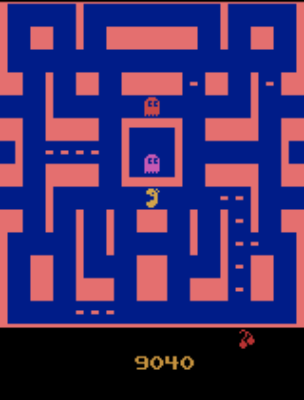
\includegraphics[width=2cm]{figures/clustering_agent_representation/pictures/ms_pacman/qualitative/cluster_2/image_1.png}
        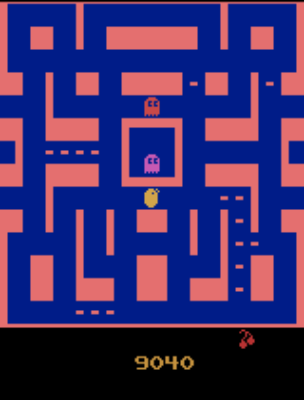
\includegraphics[width=2cm]{figures/clustering_agent_representation/pictures/ms_pacman/qualitative/cluster_2/image_2.png}

        \small End of the episode.
    \end{minipage}
    };

    \end{tikzpicture}
    }
    \caption{Clusters identified by \gls{car} in the Ms.\ Pac-Man environment (layer 6b, $K=3$).}
    \label{fig:qualitative_ms_pacman}
\end{figure}


\begin{figure}[H]
    \qualitativeClusterFigureSetup
    \qualitativeClusterTwo
        {figures/clustering_agent_representation/pictures/ms_pacman/qualitative_alt/cluster_0/image_1.png}
        {figures/clustering_agent_representation/pictures/ms_pacman/qualitative_alt/cluster_0/image_2.png}
        {D}
    \qualitativeClusterTwo
        {figures/clustering_agent_representation/pictures/ms_pacman/qualitative_alt/cluster_1/image_1.png}
        {figures/clustering_agent_representation/pictures/ms_pacman/qualitative_alt/cluster_1/image_2.png}
        {E}
    \qualitativeClusterTwo
        {figures/clustering_agent_representation/pictures/ms_pacman/qualitative_alt/cluster_2/image_1.png}
        {figures/clustering_agent_representation/pictures/ms_pacman/qualitative_alt/cluster_2/image_2.png}
        {F}
    \qualitativeClusterTwo
        {figures/clustering_agent_representation/pictures/ms_pacman/qualitative_alt/cluster_3/image_1.png}
        {figures/clustering_agent_representation/pictures/ms_pacman/qualitative_alt/cluster_3/image_2.png}
        {G}
    \qualitativeClusterTwo
        {figures/clustering_agent_representation/pictures/ms_pacman/qualitative_alt/cluster_4/image_1.png}
        {figures/clustering_agent_representation/pictures/ms_pacman/qualitative_alt/cluster_4/image_2.png}
        {H}
    \caption{Clusters D--H identified by \gls{car} in the \MsPacManName environment (layer 4, $K=5$).}
    \label{fig:qualitative_ms_pacman_alt}
\end{figure}

\vfill

\newpage
\subsection{\PongName}

Two clusterings are examined for \PongName (Table~\ref{tab:qualitative_pong_metrics}), obtained at layer 2 with $K=2$ and at layer 3 with $K=3$.

At layer 2 (Figure~\ref{fig:qualitative_pong_alt}), the partition separates the observations according to the number of digits in the player's score.
A one-digit score corresponds to cluster A.
A two-digit score corresponds to cluster B.
This reflects the progress of the game, but only through its visual display at the top of the screen.
The partition therefore captures a feature of the observation that provides no information about how the agent plays.

At layer 3 (Figure~\ref{fig:qualitative_pong}), the partition instead follows the vertical position of the ball.
The ball is at the top of the field in cluster C.
It is in the middle of the field in cluster D.
It is at the bottom of the field in cluster E.
This feature directly determines where the agent needs to place its paddle.

The clustering at layer 2 is perfectly reproducible and perfectly abstract, with \gls{cu}, \gls{as}, and \gls{acu} all equal to $1.00$.
The clustering at layer 3 is less consistent, with a \gls{cu} of $0.67$, and reaches a lower \gls{acu} of $0.65$.

\vfill
\begin{table}[H]
    \centering
    \begin{tblr}{
        width=\linewidth,
        colspec={Q[c,wd=1.6cm] X[l]},
        cells = {valign=m},
        rowsep=2pt,
        hline{1,Z} = {1pt},
        hline{4} = {0.5pt},
        hline{2,5} = {0.3pt},
        row{1,4} = {bg=black!8, font=\bfseries},
        column{1} = {font=\bfseries}
    }
        \SetCell[c=2]{l} \makebox[1.9cm][l]{Layer 2}\makebox[1.4cm][l]{$K=2$}\makebox[2.75cm][l]{\gls{cu} 1.00}\makebox[2.75cm][l]{\gls{as} 1.00}\gls{acu} 1.00 & \\
        A & The player's score has two digits. \\
        B & The player's score has one digit. \\
        \SetCell[c=2]{l} \makebox[1.9cm][l]{Layer 3}\makebox[1.4cm][l]{$K=3$}\makebox[2.75cm][l]{\gls{cu} 0.67}\makebox[2.75cm][l]{\gls{as} 0.98}\gls{acu} 0.65 & \\
        C & The ball is at the top. \\
        D & The ball is in the middle. \\
        E & The ball is at the bottom. \\
    \end{tblr}
    \caption{\gls{cu}, \gls{as}, and \gls{acu} of the two clusterings analyzed in the \PongName environment.}
    \label{tab:qualitative_pong_metrics}
\end{table}
\vfill

\newpage
\vspace*{\fill}
\begin{figure}[H]
    \qualitativeClusterFigureSetup
    \qualitativeClusterOne
        {figures/clustering_agent_representation/pictures/pong/qualitative_alt/cluster_0/image_1.png}
        {Cluster 1: paddles near the bottom.}
    \qualitativeClusterOne
        {figures/clustering_agent_representation/pictures/pong/qualitative_alt/cluster_1/image_1.png}
        {Cluster 2: paddles near the top.}
    \caption{Clusters identified by \gls{car} in the \PongName environment (layer 2, $K=2$).}
    \label{fig:qualitative_pong_alt}
\end{figure}


\begin{figure}[H]
    \qualitativeClusterFigureSetup
    \qualitativeClusterTwo
        {figures/clustering_agent_representation/pictures/pong/qualitative/cluster_0/image_1.png}
        {figures/clustering_agent_representation/pictures/pong/qualitative/cluster_0/image_2.png}
        {Cluster 1: the ball is near the bottom of the field.}
    \qualitativeClusterTwo
        {figures/clustering_agent_representation/pictures/pong/qualitative/cluster_1/image_1.png}
        {figures/clustering_agent_representation/pictures/pong/qualitative/cluster_1/image_2.png}
        {Cluster 2: the ball crosses above the opponent's paddle, left behind at the bottom.}
    \qualitativeClusterTwo
        {figures/clustering_agent_representation/pictures/pong/qualitative/cluster_4/image_1.png}
        {figures/clustering_agent_representation/pictures/pong/qualitative/cluster_4/image_2.png}
        {Cluster 3: the ball is near the top of the field, close to the player's paddle.}
    \qualitativeClusterTwo
        {figures/clustering_agent_representation/pictures/pong/qualitative/cluster_2/image_1.png}
        {figures/clustering_agent_representation/pictures/pong/qualitative/cluster_2/image_2.png}
        {Cluster 4: same as cluster 1.}
    \qualitativeClusterTwo
        {figures/clustering_agent_representation/pictures/pong/qualitative/cluster_3/image_1.png}
        {figures/clustering_agent_representation/pictures/pong/qualitative/cluster_3/image_2.png}
        {Cluster 5: same as cluster 2.}
    \qualitativeClusterTwo
        {figures/clustering_agent_representation/pictures/pong/qualitative/cluster_5/image_1.png}
        {figures/clustering_agent_representation/pictures/pong/qualitative/cluster_5/image_2.png}
        {Cluster 6: same as cluster 3.}
    \caption{Clusters identified by \gls{car} in the \PongName environment (layer 4, $K=6$). Clusters 4--6 duplicate the semantics of clusters 1--3, illustrating over-segmentation at this value of $K$.}
    \label{fig:qualitative_pong}
\end{figure}

\vfill

\newpage
\subsection{\SpaceInvadersName}

Two clusterings are examined for \SpaceInvadersName (Table~\ref{tab:qualitative_space_invaders_metrics}), obtained at layer 4 with $K=4$ and at layer 2 with $K=5$.

At layer 4 (Figure~\ref{fig:qualitative_space_invaders}), the partition tracks the progression of the episode.
The start of the episode is captured in (cluster D).
The middle of the episode is captured in (cluster B).
The end of the episode is captured in (cluster C).
A specific behavior in which the agent has cleared the leftmost column and is positioned to catch the flying saucer that occasionally crosses the top of the screen is captured in (cluster A).

At layer 2 (Figure~\ref{fig:qualitative_space_invaders_alt}), the partition again tracks the progression of the episode.
The start of the episode is captured in (cluster G).
The middle of the episode is captured in (cluster F).
The end of the episode is captured in (cluster I).
Attacking the first two columns of the formation is captured in (cluster E).
Trying to catch the flying saucer is captured in (cluster H).

The clustering at layer 4 has a \gls{cu} of $0.92$ and a \gls{as} of $0.69$, resulting in a \gls{acu} of $0.61$.
The clustering at layer 2 has the same \gls{cu} of $0.92$, but a lower \gls{as} of $0.49$, resulting in a lower \gls{acu} of $0.41$.

\vfill
\begin{table}[H]
    \centering
    \begin{tblr}{
        width=\linewidth,
        colspec={Q[c,wd=1.6cm] X[l]},
        cells = {valign=m},
        rowsep=2pt,
        hline{1,Z} = {1pt},
        hline{6} = {0.5pt},
        hline{2,7} = {0.3pt},
        row{1,6} = {bg=black!8, font=\bfseries},
        column{1} = {font=\bfseries}
    }
        \SetCell[c=2]{l} \makebox[1.9cm][l]{Layer 4}\makebox[1.4cm][l]{$K=4$}\makebox[2.75cm][l]{\gls{cu} 0.92}\makebox[2.75cm][l]{\gls{as} 0.69}\gls{acu} 0.61 & \\
        A & The left column has been cleared; the flying saucer occasionally appears. \\
        B & Middle of the episode. \\
        C & End of the episode. \\
        D & Start of the episode. \\
        \SetCell[c=2]{l} \makebox[1.9cm][l]{Layer 2}\makebox[1.4cm][l]{$K=5$}\makebox[2.75cm][l]{\gls{cu} 0.92}\makebox[2.75cm][l]{\gls{as} 0.49}\gls{acu} 0.41 & \\
        E & Attacks the first two columns of the formation. \\
        F & Middle of the episode. \\
        G & Start of the episode. \\
        H & Tries to catch the flying saucer. \\
        I & End of the episode. \\
    \end{tblr}
    \caption{\gls{cu}, \gls{as}, and \gls{acu} of the two clusterings analyzed in the \SpaceInvadersName environment.}
    \label{tab:qualitative_space_invaders_metrics}
\end{table}
\vfill

\newpage
\vspace*{\fill}
\begin{figure}[H]
    \qualitativeClusterFigureSetup
    \qualitativeClusterTwo
        {figures/clustering_agent_representation/pictures/space_invaders/qualitative/cluster_3/image_1.png}
        {figures/clustering_agent_representation/pictures/space_invaders/qualitative/cluster_3/image_2.png}
        {Start of the episode.}
    \qualitativeClusterTwo
        {figures/clustering_agent_representation/pictures/space_invaders/qualitative/cluster_1/image_1.png}
        {figures/clustering_agent_representation/pictures/space_invaders/qualitative/cluster_1/image_2.png}
        {Middle of the episode.}
    \qualitativeClusterTwo
        {figures/clustering_agent_representation/pictures/space_invaders/qualitative/cluster_0/image_1.png}
        {figures/clustering_agent_representation/pictures/space_invaders/qualitative/cluster_0/image_2.png}
        {The left column has been cleared; the flying saucer occasionally appears.}
    \qualitativeClusterTwo
        {figures/clustering_agent_representation/pictures/space_invaders/qualitative/cluster_2/image_1.png}
        {figures/clustering_agent_representation/pictures/space_invaders/qualitative/cluster_2/image_2.png}
        {Late in the episode, few invaders remain.}
    \caption{Clusters identified by \gls{car} in the \SpaceInvadersName environment (layer 4, $K=4$).}
    \label{fig:qualitative_space_invaders}
\end{figure}


\begin{figure}[H]
    \qualitativeClusterFigureSetup
    \qualitativeClusterOne
        {figures/clustering_agent_representation/pictures/space_invaders/qualitative_alt/cluster_0/image_1.png}
        {Cluster 1: formation nearly intact.}
    \qualitativeClusterOne
        {figures/clustering_agent_representation/pictures/space_invaders/qualitative_alt/cluster_1/image_1.png}
        {Cluster 2: formation partially thinned.}
    \qualitativeClusterOne
        {figures/clustering_agent_representation/pictures/space_invaders/qualitative_alt/cluster_2/image_1.png}
        {Cluster 3: formation reorganized, three lives left.}
    \qualitativeClusterOne
        {figures/clustering_agent_representation/pictures/space_invaders/qualitative_alt/cluster_3/image_1.png}
        {Cluster 4: left column cleared, flying saucer visible.}
    \qualitativeClusterOne
        {figures/clustering_agent_representation/pictures/space_invaders/qualitative_alt/cluster_4/image_1.png}
        {Cluster 5: formation reduced to two columns.}
    \caption{Clusters identified by \gls{car} in the \SpaceInvadersName environment (layer 2, $K=5$).}
    \label{fig:qualitative_space_invaders_alt}
\end{figure}

\vfill

\newpage
\subsection{\SurroundName}

Two clusterings are examined for \SurroundName (Table~\ref{tab:qualitative_surround_metrics}), obtained at layer 8b with $K=4$ and at layer 7b with $K=6$.

At layer 8b (Figure~\ref{fig:qualitative_surround}), the partition captures the start of the episode in cluster B.
The outcome of the episode, when the opponent loses, is captured in cluster D.
The player's trail is confined to the bottom-left area in cluster A.
The player reaches the top of the level from the left and then moves along the top in cluster C.

At layer 7b (Figure~\ref{fig:qualitative_surround_alt}), the partition again captures the start of the episode in cluster J.
The outcome of the episode, when the opponent loses, is captured in cluster F.
The player moves in the upper-left corner in cluster E.
The player moves in the lower-left corner in cluster G.
The end of the game is played in the lower-left corner in cluster H.
The player crosses the level from the top left to the bottom right in cluster I.

The clustering at layer 8b has a \gls{cu} of $0.67$, a \gls{as} of $0.71$, and a \gls{acu} of $0.38$.
The clustering at layer 7b reaches the same values, with a \gls{cu} of $0.67$, a \gls{as} of $0.71$, and a \gls{acu} of $0.38$.

\vfill
\begin{table}[H]
    \centering
    \begin{tblr}{
        width=\linewidth,
        colspec={Q[c,wd=1.6cm] X[l]},
        cells = {valign=m},
        rowsep=2pt,
        hline{1,Z} = {1pt},
        hline{6} = {0.5pt},
        hline{2,7} = {0.3pt},
        row{1,6} = {bg=black!8, font=\bfseries},
        column{1} = {font=\bfseries}
    }
        \SetCell[c=2]{l} \makebox[1.9cm][l]{Layer 8b}\makebox[1.4cm][l]{$K=4$}\makebox[2.75cm][l]{\gls{cu} 0.67}\makebox[2.75cm][l]{\gls{as} 0.71}\gls{acu} 0.38 & \\
        A & The agent's trail remains confined to the bottom-left area. \\
        B & Start of the episode. \\
        C & The agent moves along the top of the level, arriving from the left. \\
        D & The opponent loses by running into a trail. \\
        \SetCell[c=2]{l} \makebox[1.9cm][l]{Layer 7b}\makebox[1.4cm][l]{$K=6$}\makebox[2.75cm][l]{\gls{cu} 0.67}\makebox[2.75cm][l]{\gls{as} 0.71}\gls{acu} 0.38 & \\
        E & The player moves in the upper-left corner. \\
        F & The opponent loses the confrontation. \\
        G & The player moves in the lower-left corner. \\
        H & The end of the game is played in the lower-left corner. \\
        I & The player starts at the top left and ends at the bottom right. \\
        J & Start of the episode. \\
    \end{tblr}
    \caption{\gls{cu}, \gls{as}, and \gls{acu} of the two clusterings analyzed in the \SurroundName environment.}
    \label{tab:qualitative_surround_metrics}
\end{table}
\vfill

\newpage
\vspace*{\fill}
\begin{figure}[H]
    \qualitativeClusterFigureSetup
    \qualitativeClusterTwo
        {figures/clustering_agent_representation/pictures/surround/qualitative/cluster_1/image_1.png}
        {figures/clustering_agent_representation/pictures/surround/qualitative/cluster_1/image_2.png}
        {Start of the episode.}
    \qualitativeClusterTwo
        {figures/clustering_agent_representation/pictures/surround/qualitative/cluster_0/image_1.png}
        {figures/clustering_agent_representation/pictures/surround/qualitative/cluster_0/image_2.png}
        {The agent's trail remains confined to the bottom-left area.}
    \qualitativeClusterTwo
        {figures/clustering_agent_representation/pictures/surround/qualitative/cluster_2/image_1.png}
        {figures/clustering_agent_representation/pictures/surround/qualitative/cluster_2/image_2.png}
        {The agent moves along the top of the level, arriving from the left.}
    \qualitativeClusterTwo
        {figures/clustering_agent_representation/pictures/surround/qualitative/cluster_3/image_1.png}
        {figures/clustering_agent_representation/pictures/surround/qualitative/cluster_3/image_2.png}
        {The trail grows from the top-left toward the bottom, closing in on the final enclosure.}
    \caption{Clusters identified by \gls{car} in the \SurroundName environment (layer 8b, $K=4$).}
    \label{fig:qualitative_surround}
\end{figure}


\begin{figure}[H]
    \qualitativeClusterFigureSetup
    \qualitativeClusterTwo
        {figures/clustering_agent_representation/pictures/surround/qualitative_alt/cluster_0/image_1.png}
        {figures/clustering_agent_representation/pictures/surround/qualitative_alt/cluster_0/image_2.png}
        {E}
    \qualitativeClusterTwo
        {figures/clustering_agent_representation/pictures/surround/qualitative_alt/cluster_1/image_1.png}
        {figures/clustering_agent_representation/pictures/surround/qualitative_alt/cluster_1/image_2.png}
        {F}
    \qualitativeClusterTwo
        {figures/clustering_agent_representation/pictures/surround/qualitative_alt/cluster_2/image_1.png}
        {figures/clustering_agent_representation/pictures/surround/qualitative_alt/cluster_2/image_2.png}
        {G}
    \qualitativeClusterTwo
        {figures/clustering_agent_representation/pictures/surround/qualitative_alt/cluster_3/image_1.png}
        {figures/clustering_agent_representation/pictures/surround/qualitative_alt/cluster_3/image_2.png}
        {H}
    \qualitativeClusterTwo
        {figures/clustering_agent_representation/pictures/surround/qualitative_alt/cluster_4/image_1.png}
        {figures/clustering_agent_representation/pictures/surround/qualitative_alt/cluster_4/image_2.png}
        {I}
    \qualitativeClusterTwo
        {figures/clustering_agent_representation/pictures/surround/qualitative_alt/cluster_5/image_1.png}
        {figures/clustering_agent_representation/pictures/surround/qualitative_alt/cluster_5/image_2.png}
        {J}
    \caption{Clusters E--J identified by \gls{car} in the \SurroundName environment (layer 7b, $K=6$).}
    \label{fig:qualitative_surround_alt}
\end{figure}

\vfill


\section{Conclusion}
\label{sec:experiments_conclusion}

The experiments reported in this chapter apply \gls{car} and its metrics to five Atari environments.
The surrogate policies reproduce the behavior of the initial policies with an average \BehaviorReconstructionName of $0.94 \pm 0.02$.
The latent clusterings are stable across independently trained surrogate policies, with a \ClusteringUniversalityName of about $0.5$ from three clusters onward, and they are largely independent of the observation and action spaces, with an average \AbstractionScoreName of $0.99 \pm 0.00$.
Together, these results provide empirical support for the \RepresentationConvergenceHypothesisName and, more broadly, for the hypothesis-driven approach underlying \gls{car}.

Several methodological choices have not yet been evaluated.
These include the \gls{nn} architecture, the layer selected for analysis, the distance used to compare embeddings, and the clustering algorithm.
Their impact should be studied jointly to determine how much the discovered \gls{cs} depends on the analysis procedure rather than on the policy itself.

The evaluation is also limited in scope.
It considers only five Atari games, and the semantic labels attached to the clusters in Figure~\ref{fig:semantic_granularity} were assigned by hand, which is time-consuming and subjective.
Extending the study to more diverse environments and developing human-centered evaluation protocols would strengthen the validity of the resulting explanations.

